%--------------------------------------------------------------------
%--------------------------------------------------------------------
% Formato para los talleres del curso de Métodos Computacionales
% Universidad de los Andes
%--------------------------------------------------------------------
%--------------------------------------------------------------------

\documentclass[11pt,letterpaper]{exam}
\usepackage[utf8]{inputenc}
\usepackage[spanish]{babel}
\usepackage{graphicx}
\usepackage{tabularx}
\usepackage[absolute]{textpos} % Para poner una imagen en posiciones arbitrarias
\usepackage{multirow}
\usepackage{float}
\usepackage{hyperref}
%\decimalpoint

\begin{document}
\begin{center}
{\Large Métodos Computacionales} \\
\textsc{Tarea 2}\\
01-2019\\
\end{center}

\noindent
\section{Ejercicio 1: Fourier}
\subsection{Gráfica señales}
\begin{figure}[H]
\centering
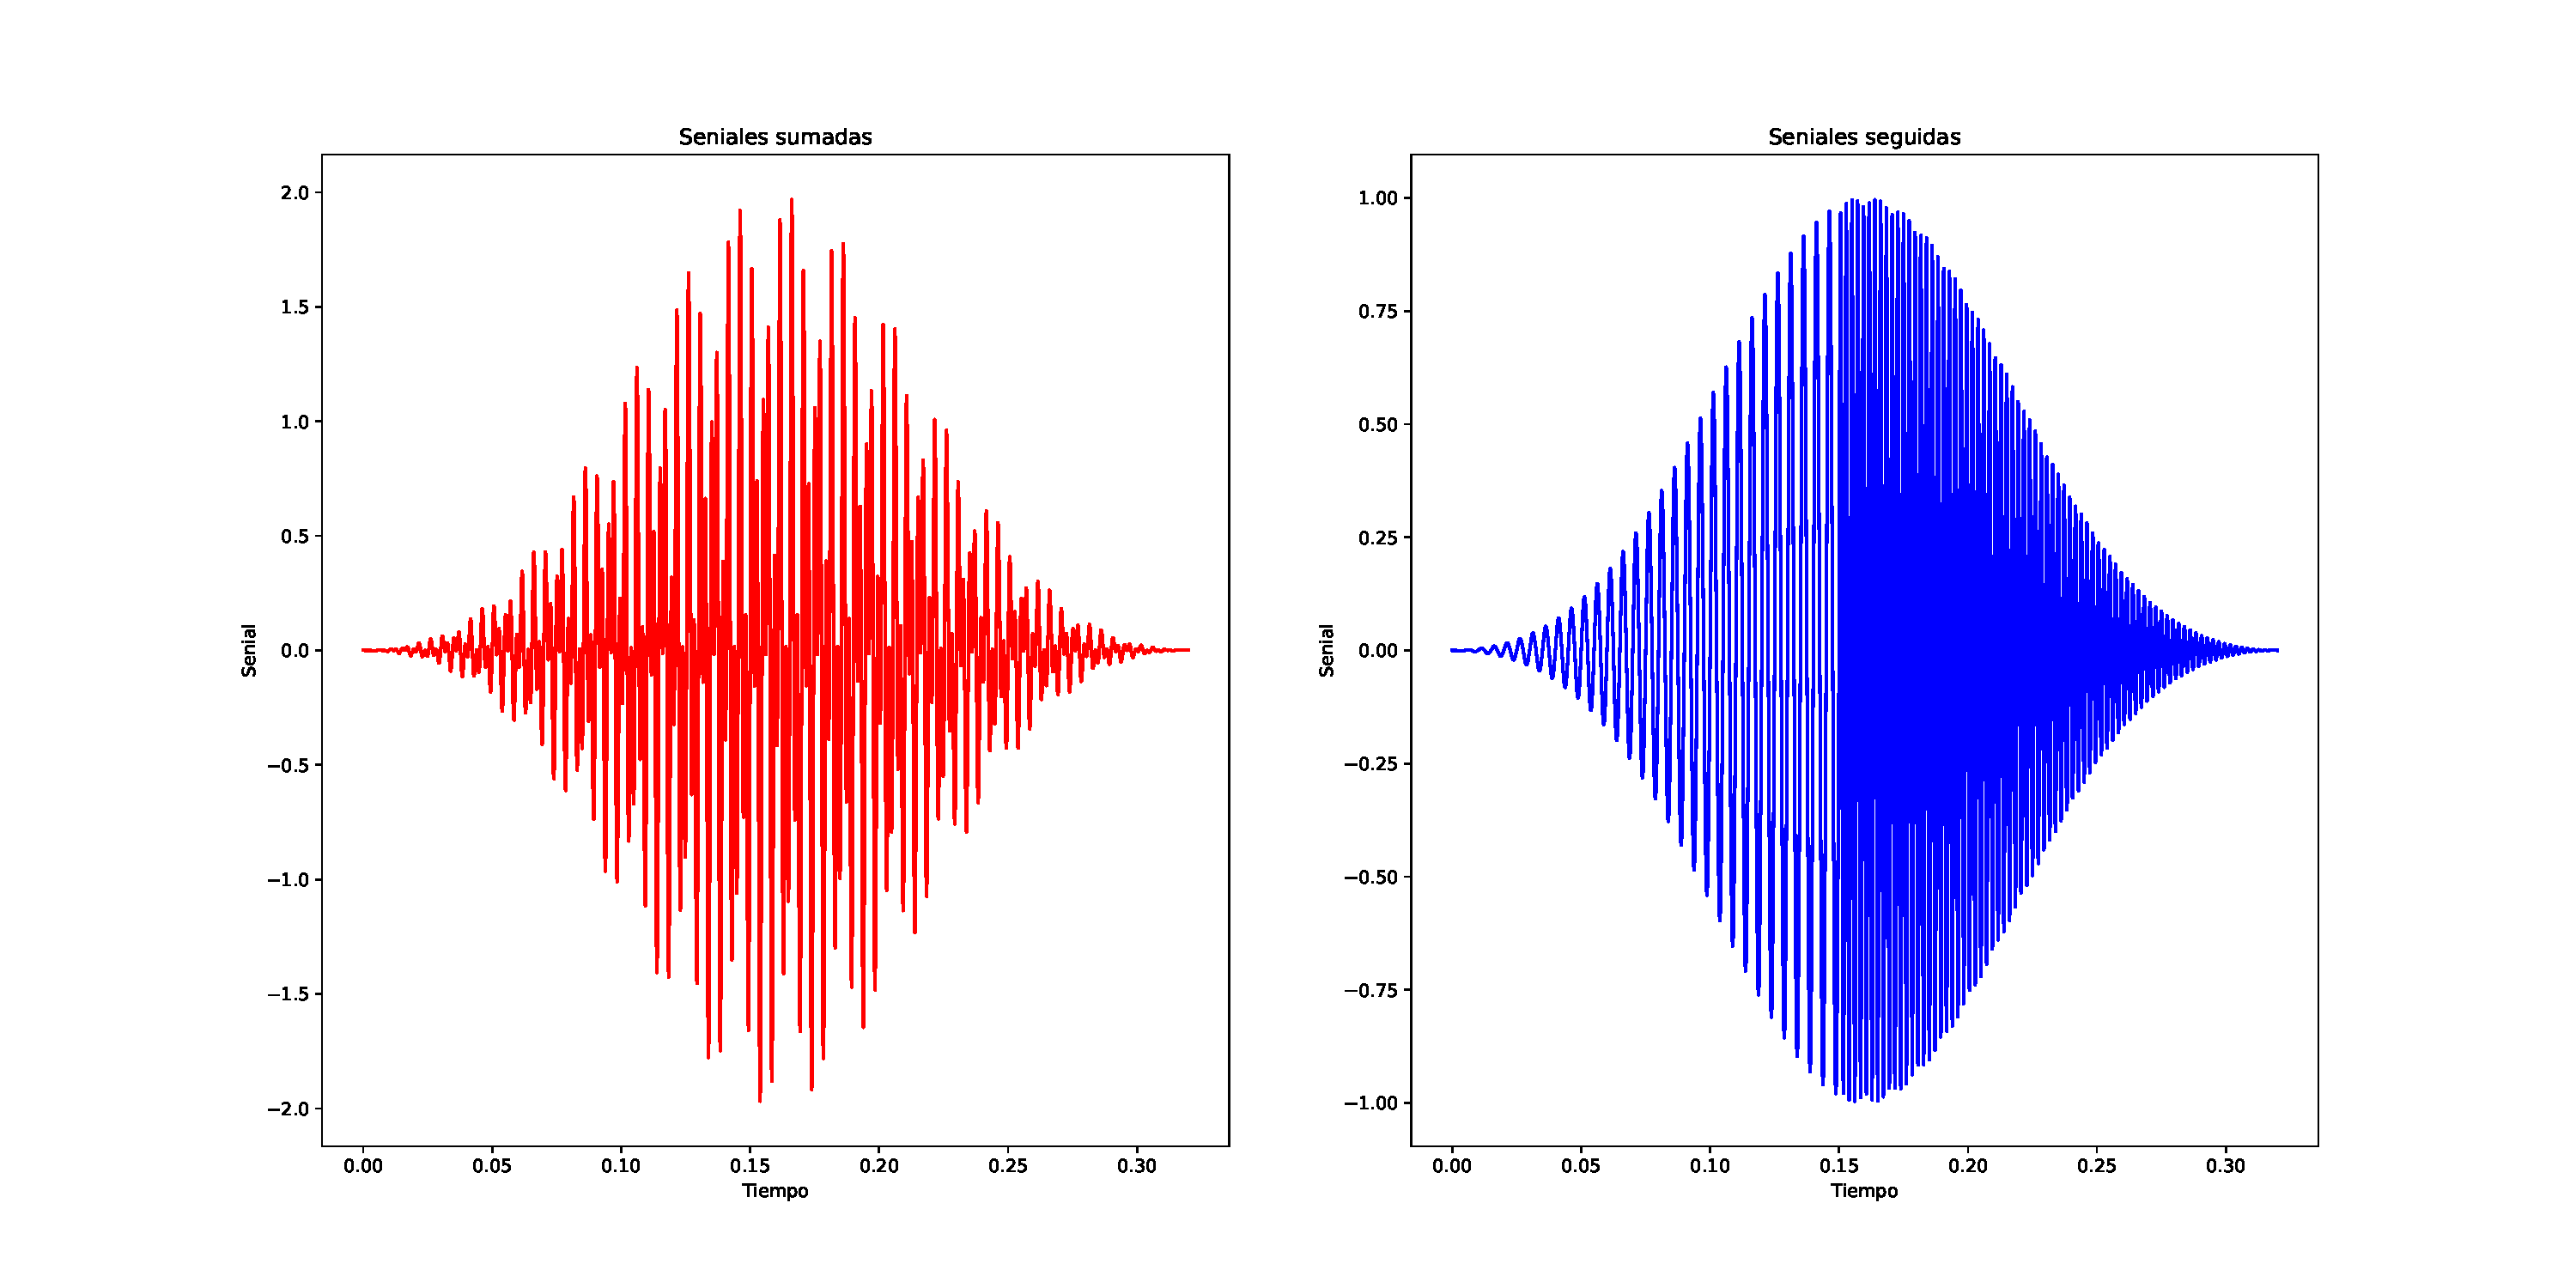
\includegraphics[scale=0.35]{PlotFourier1.pdf}
\end{figure}

\subsection{Gráfica señales transformadas}
\begin{figure}[H]
\centering
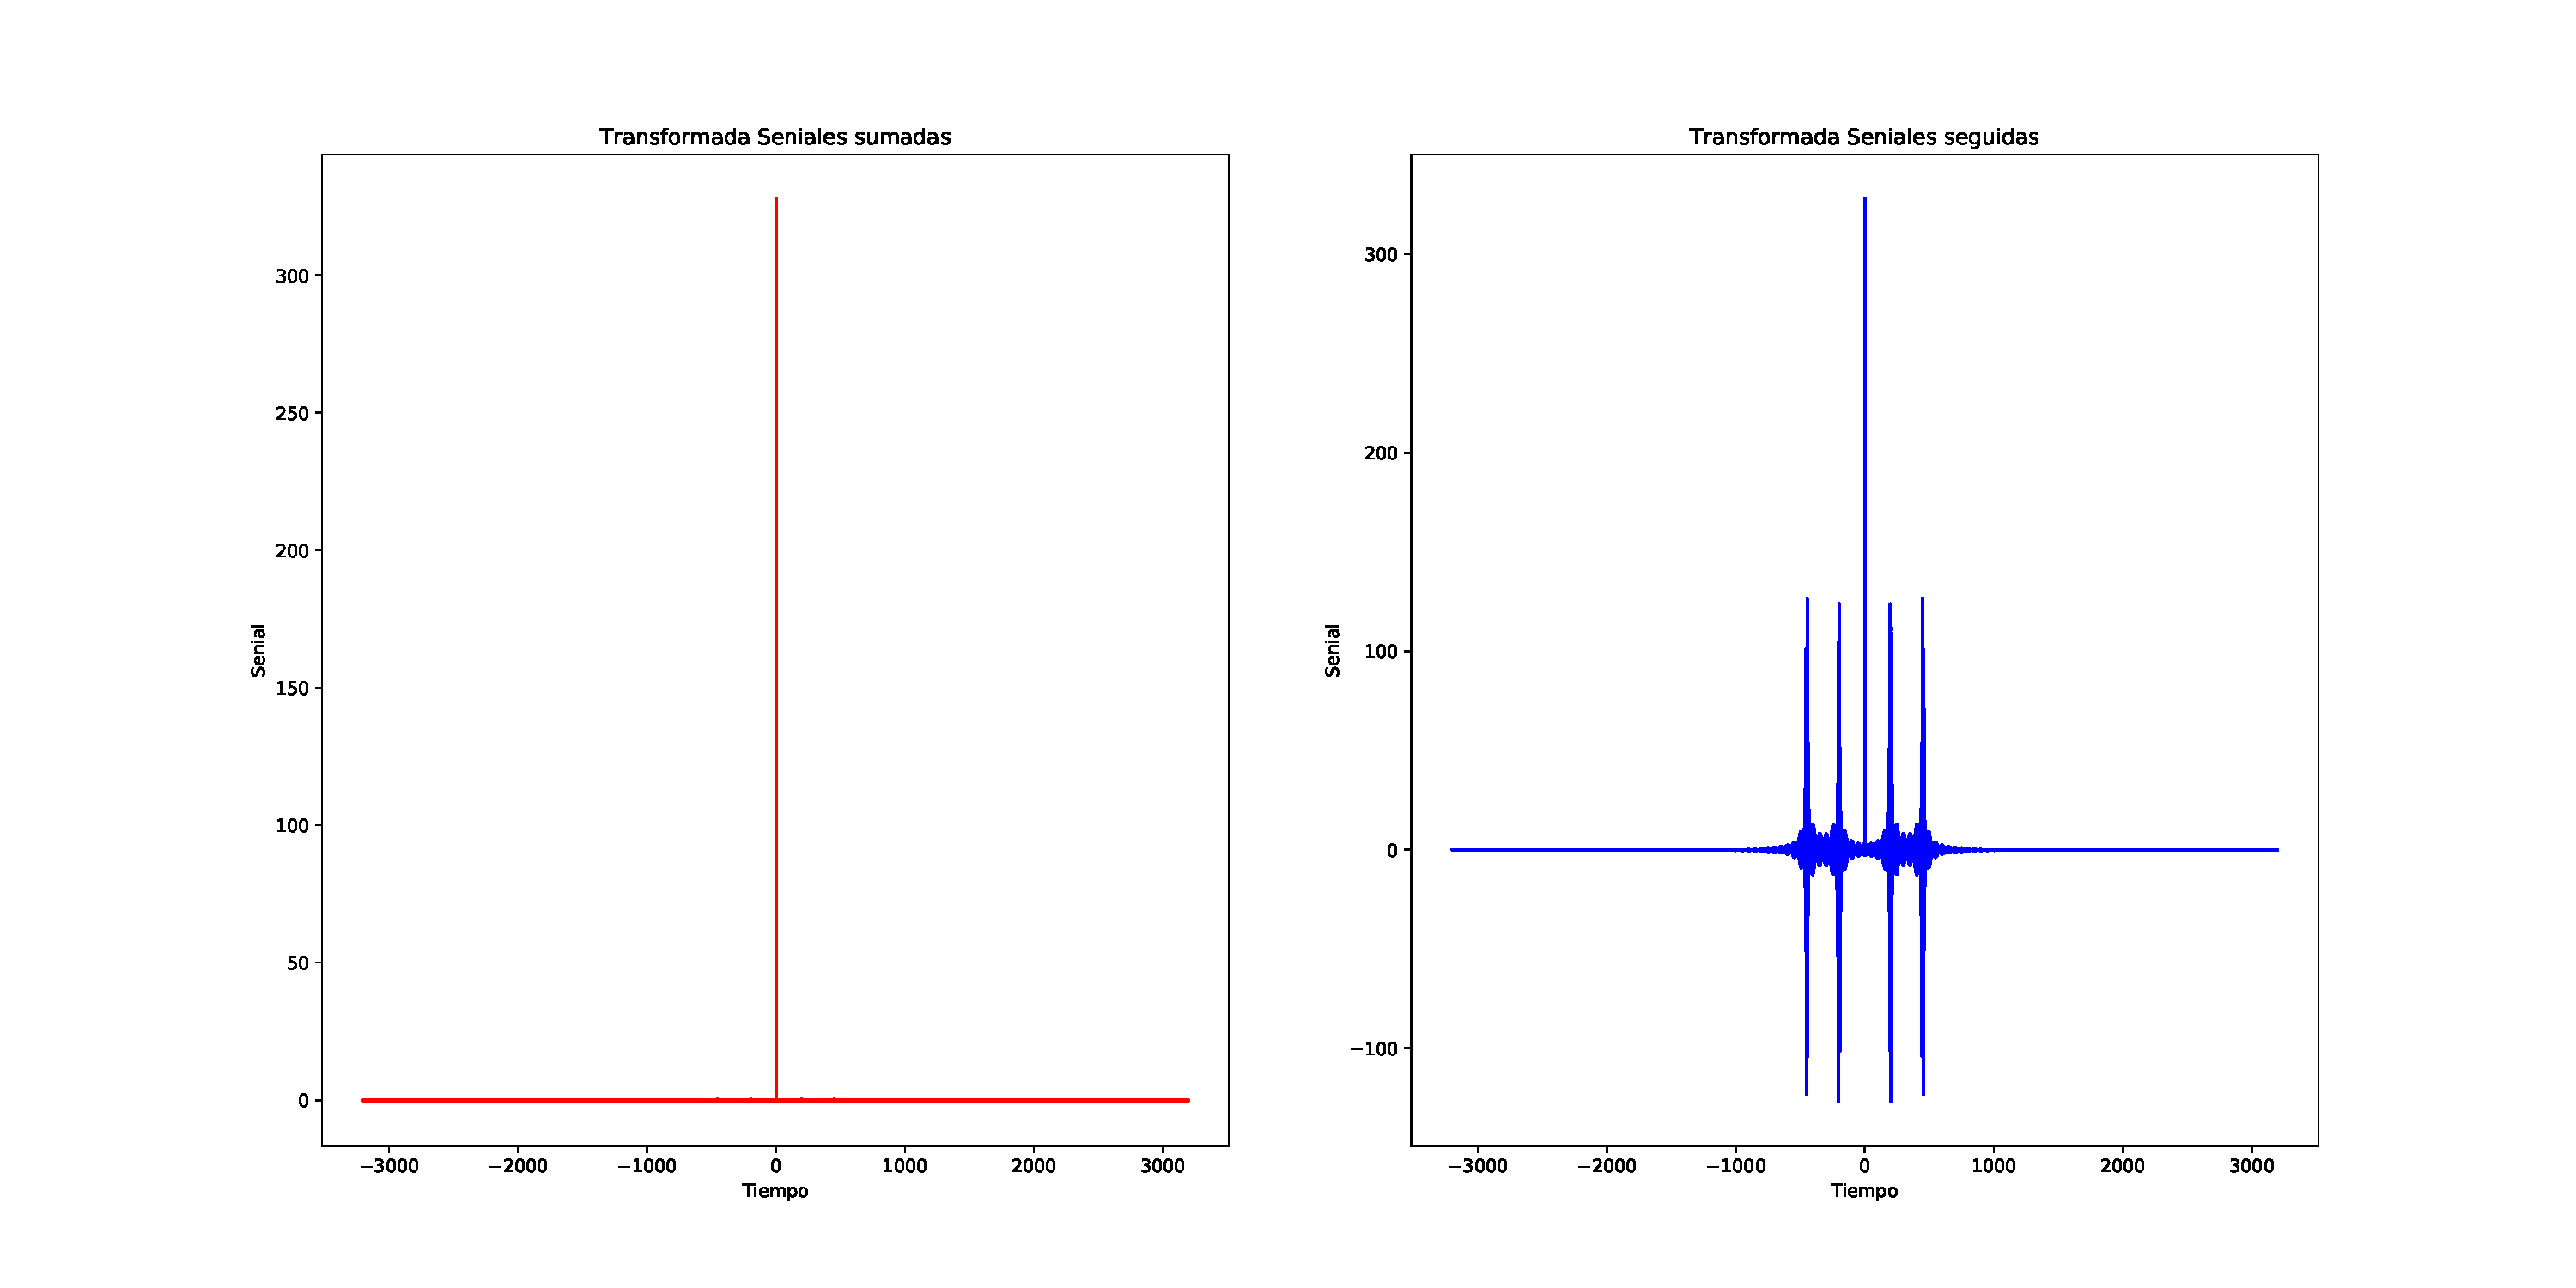
\includegraphics[scale=0.35]{PlotTransFourier2.pdf}
\end{figure}
Coherente con la solucion analitica de aplicar la transformada de Fourier a unas señales con la forma funcional de las señales dadas, ambas gráficas exhiben 4 picos.  

\subsection{Espectrograma señal sumada}
\begin{figure}[H]
\centering
\includegraphics[scale=0.75]{specgram1.pdf}
\end{figure}
El espectrograma muestra que para el caso en que se suman las ondas a diferentes frecuencias, en efecto se tienen dos frecuencias constantes durante todo el tiempo que dura la señal. Puede verse que es la suma de dos ondas, una con el doble de frecuencia a la otra.
\subsection{Espectrograma señal seguida}
\begin{figure}[H]
\centering
\includegraphics[scale=0.75]{specgram2.pdf}
\end{figure}
El espectrograma muestra que para este caso que la primera mitad del tiempo la señal es de una onda a una frecuencia, y luego la frecuencia se duplica. Puede verse que hacia t=10 el espectrograma muestra un salto en la frecuencia.
\subsection{Gráfica señal temblor}
\begin{figure}[H]
\centering
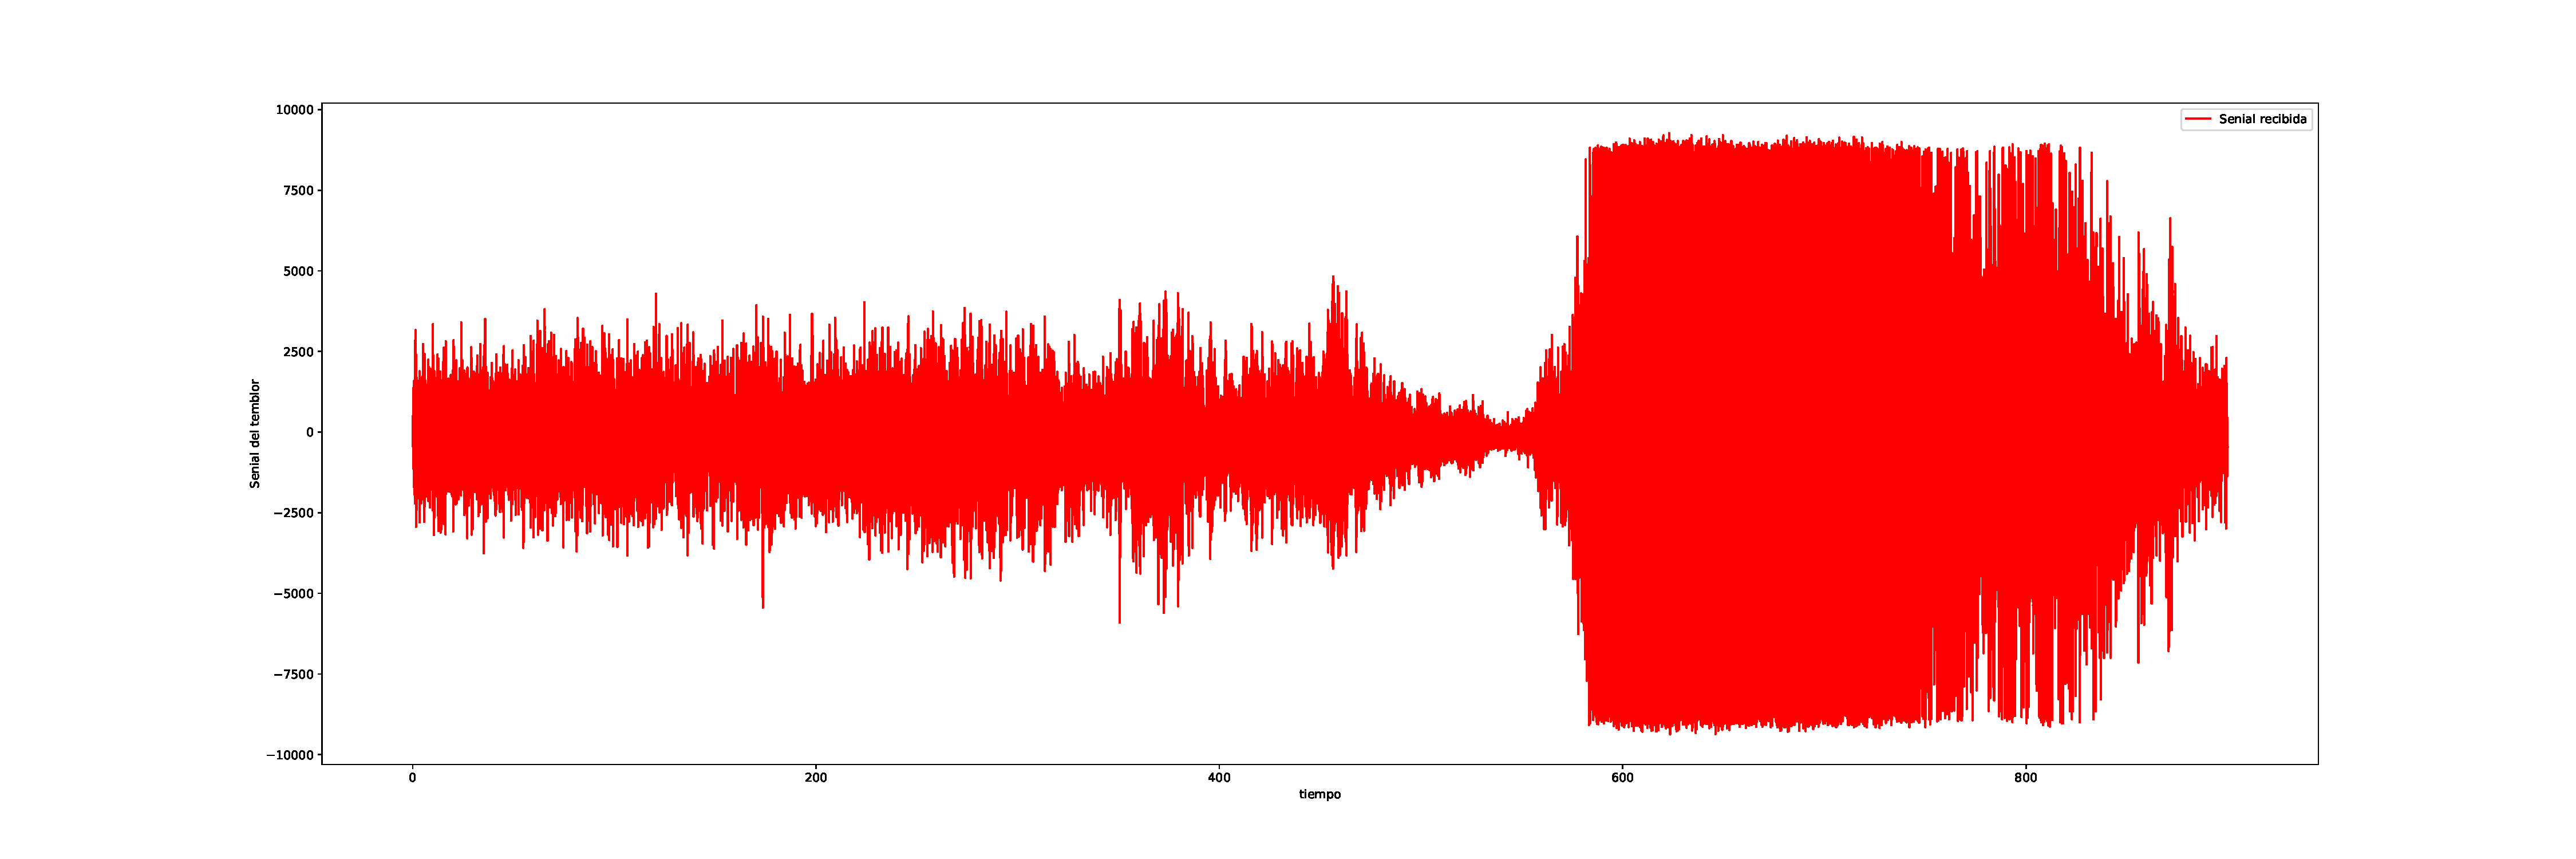
\includegraphics[scale=0.25]{PlotFourier3.pdf}
\end{figure}
Puede decirse que hacia poco antes del tiempo t=600 es que empieza el temblor, caracterizado por un incremento súbito en la amplitud de la señal.

\subsection{Gráfica señal temblor transformada}
\begin{figure}[H]
\centering
\includegraphics[scale=0.25]{PlotFourier4.pdf}
\end{figure}
Puede verse que el temblor está caracterizado por movimientos de alta frecuencia y gran amplitud.

\subsection{Espectrograma señal temblor}
\begin{figure}[H]
\centering
\includegraphics[scale=0.75]{specgramTemblor.pdf}
\end{figure}
Puede verse que en efecto la frecuencia se dipara hacia poco antes de t=600, lo que es indicio de que en ese momento inicia el temblor.

\section{Ejercicio 2: ODEs}
\subsection{Amplitudes maximas en función de la frecuencia}
\begin{figure}[H]
\centering
\includegraphics[scale=0.4]{UF.pdf}
\end{figure}
Puede verse que, en coherencia con un modelo de 3 resortes y 3 masas, se encuentran 3 frecuencias de resonancia, caracterizados por los tres picos que se exhiben para todos los pisos, en la misma frecuencia. 

\subsection{Frecuencias de interés}
Se escogieron las frecuencias donde se exhibían los picos (las de resonancia), y un punto por encima de los 2 Hz donde las 3 frecuencias se hacen casi iguales.\\
Se escogen los que generan los picos: $\omega$=0.639225; $\omega$=1.74797;  $\omega$=2.53993. Y el en el que son más similares los máximos: $\omega$=2.10435.
\begin{figure}[H]
\centering
\includegraphics[scale=0.8]{w9.pdf}
\end{figure}

\begin{figure}[H]
\centering
\includegraphics[scale=0.8]{w37.pdf}
\end{figure}

\begin{figure}[H]
\centering
\includegraphics[scale=0.8]{w57.pdf}
\end{figure}

En las tres gráficas anteriores se tiene la amplitud del movimiento de los pisos en función del tiempo para un temblor que oscile en con la frecuencia de resonancia del edificio. Como se puede ver, la amplitud es creciente en el tiempo de exposición al forzamiento del temblor en la frecuencia de resonancia. Esto significa que, una exposición larga a un temblor que produzca oscilaciones en la fecuencia de resonancia del edificio puede acabar derrumbándolo.

\begin{figure}[H]
\centering
\includegraphics[scale=0.8]{w46.pdf}
\end{figure}
Esta frecuencia pareció interesante porque los máximos de amplitud era muy similar en todos los pisos. Como se puede ver, a esta frecuencia, parece que todos los pisos exhiben una vibración que recuerda a ondas superpuestas. (SIGUE, SE HIZO EL BONO)

\section{BONO:}
\begin{figure}[H]
\centering
\includegraphics[scale=0.4]{BONO.pdf}
\caption{Rojo: edificios de entre 3 y 9 pisos; Azul: edificios de entre 10 y 16 pisos; Verde edificios de entre 17 y 22 pisos}
\end{figure}
Para el bono se decidió estudiar
\end{document}